\chapter{Architectuur}\label{ch:Architectuur}

Om inzicht te verkrijgen in potentiële kwetsbaarheden in de projecten van Eaglescience moet er een applicatie worden ontworpen die analyses kan uitvoeren op het moment dat er veranderingen worden aangebracht in deze projecten. Daarnaast moet de applicatie in staat zijn deze analyses uit te voeren op een periodieke basis.
Op het moment van schrijven wordt er binnen Eaglescience ontwikkeld in de talen Scala en TypeScript, maar de verwachting is dat er in de toekomst een mogelijkheid bestaat dat dit uitgebreid gaat worden. Daarnaast zijn deze twee talen niet de enige twee platformen binnen de stack, maar wordt er ook gebruik gemaakt van docker met daarbij verschillende images die ook kwetsbaarheden kunnen bevatten. Dit ontwerp voorziet niet in de mogelijkheid om deze toekomstige platformen (als Docker) te kunnen scannen, echter zal het wel de mogelijkheid bieden om deze op een relatief makkelijke manier later toe te voegen. De selectie van deze toekomstige tool moet wel de mogelijkheid bieden om te voorzien in de data beschreven in het interne datamodel.

Analyses worden uitgevoerd op module niveau, hier zijn in basis twee redenen voor. Ten eerste is een module binnen een Eaglescience project een afgeschermd onderdeel dat een eigen platform benut. Ten tweede kunnen er op module niveau veranderingen worden verwacht ten opzichte van dependency declaraties.

Als de architectuur wordt gebasseerd op het datamodel kan er vervolgens worden gekeken welke componenten en technieken er nodig zijn om het datamodel functioneeel te krijgen.

\section{Datamodel}\label{subsec:datamodel}
Het datamodel is opgebouwd op basis van de data die wordt verkregen van de in het onderzoek gevonden OWASP tools. Hieruit kan worden gedestileerd welke gegevens daadwerkelijk nodig zijn voor de functionaliteit die wordt verwacht binnen Eaglescience. Het in figuur~\ref{fig:SOUP-SoupApiDm} getoonde model laat deze destillatie zien. Centraal in het datamodel staat de analyse. De analyse is aan modules gekoppeld omdat de rapportages uit de SCA tooling gebasseerd zijn op modules en niet op projecten. Het project is een verzameling modules dat in zijn geheel een applicatie vormt. De analyse zelf is opgebouwd uit de dependency files, welke opgeslagen worden om in de toekomst periodieke analyses uit te kunnen voeren tot er een nieuwe analyse is. Ook worden alle dependencies opgeslagen waarin gevonden vulnarabilities en bewijs worden opgeslagen.

\begin{figure}[H]
    \myfloatalign
    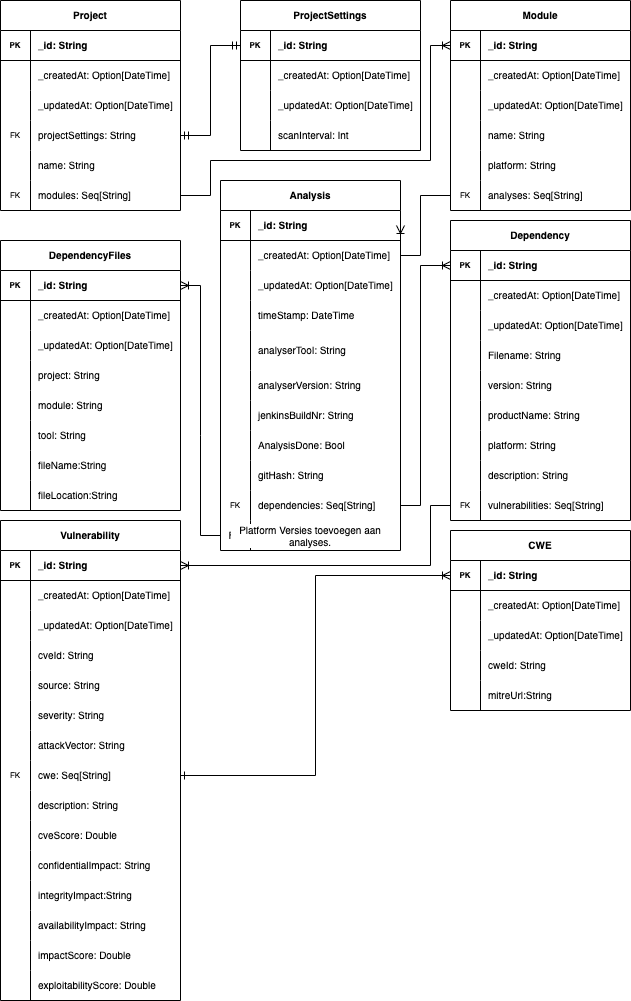
\includegraphics[width=12cm]{gfx/SOUPAPI-SOUPAPI DM}
    \caption{Intern Datamodel}
    \label{fig:SOUP-SoupApiDm}
\end{figure}

Hieronder wordt iedere entiteit beschreven met daarin het attribuut, het datatype en de reden voor het opslaan van deze data, waarbij geldt dat voor iedere entititeit de volgende attributen standaard zijn \_id, \_createdAt en \_updatedAt opgeslagen.

\begin{tabular}{lll}
    \textbf{Attribuut} & \textbf{Datatype} & \textbf{notitie}\\
    \_id & String & unique primary key\\
    \_createdAt & DateTime & timestamp aanmaken van record\\
    \_updatedAt & DateTime & timestampt wijzigen van record\\

\end{tabular}
%TODO dit is leidend datamodel bijwerken.
\subsection{Project}\label{subsec:project}
In deze entititeit worden de basisgegevens van de projecten opgeslagen als ook de relaties met de voor ieder project aanwezige modulen.

\begin{tabular}{lll}
    \textbf{Attribuut} & \textbf{Datatype} & \textbf{notitie}\\
    projectSettings & String & referentie naar projectsettings\\
    name & String & naam van het project\\
    modules & Seq[String] & bij project horende modules\\

\end{tabular}
\subsection{Projectsettings}\label{subsec:projectsettings}
Deze enititeit geeft de mogelijkheid tot het opslaan van project specifieke instellingen met betrekking tot de SOUP API.

\begin{tabular}{lll}
    \textbf{Attribuut} & \textbf{Datatype} & \textbf{notitie}\\
    scaninterval  & String & aantal dagen tussen analyses\\
\end{tabular}

\subsection{Module}\label{subsec:module}
De module is een op zichzelf staand onderdeel van de applicatie geisoleerd door een platform en de specifieke functie. Er kunnen meerdere modules in een project zitten.

\begin{tabular}{lll}
    \textbf{Attribuut} & \textbf{Datatype} & \textbf{notitie}\\
    name  & String & naam van de module\\
    platform  & String & platform waar de module op geschreven is \\
    analyses  & Seq[String] & reverentie naar alle analyses die gedaan zijn op de module\\
\end{tabular}

\subsection{Analysis}\label{subsec:analysis}
Een analyse herbergt alle bekende informatie over een module op het moment van de analyse. De dependencies die hier opgeslagen zijn zijn de op dat moment aanwezige dependencies in de module waar de analyse op plaats heeft gevonden. De dependecyfiles worden ook opgeslagen om een periodieke analyse mogelijk te maken op de module die op dat moment bestaat.

\begin{tabular}{lll}
    \textbf{Attribuut} & \textbf{Datatype} & \textbf{notitie}\\
    timeStamp & DateTime & naam van de module\\
    analyserTool & String & naam van de analyser tool\\
    analyserEngine & String & versie van de SCA tool die gebruikt is\\
    jenkinsBuildNr & Int & JenkinsBuildnr tracebility naar Jenkins\\
    gitHash & String & Githash van een analyseerde module Tracability naar Gitlab\\
    dependencies & Seq[String] & reverentie naar alle dependendencies in de module\\
    dependencyFiles & Seq[String] & reverentie naar alle dependencyFiles gedefinieerd in de module\\
\end{tabular}


\subsection{Dependency}\label{subsec:dependency}
%TODO tot hier gekomen
\begin{tabular}{lll}
    \textbf{Attribuut} & \textbf{Datatype} & \textbf{notitie}\\
    timeStamp & DateTime & naam van de module\\
    analyserTool & String & Naam van de analyser tool\\
    analyserEngine & String & Versie van de SCA tool die gebruikt is\\
    jenkinsBuildNr & Int & JenkinsBuildnr tracebility naar Jenkins\\
    gitHash & String & Githash van  eanalyseerde module Tracability naar Gitlab\\
    dependencies & Seq[String] & Reverentie naar alle dependendencies in de module.\\
    dependencyFiles & Seq[String] & Reverentie naar alle dependencyFiles gedifineerd in de module.\\
    nodeversion & String & versie van Node  \\
    npmversion & String & versie van NPM  \\
    sbtversion & String & versie van Version  \\
    scalaversion & String & versie van scala  \\
    javaversion & String & versie van java \\
\end{tabular}

\subsection{DependencyFiles}\label{subsec:dependencyFiles}
\begin{tabular}{lll}
    \textbf{Attribuut} & \textbf{Datatype} & \textbf{notitie}\\
    nodeversion & String & versie van Node  \\
    npmversion & String & versie van NPM  \\
    sbtversion & String & versie van Version  \\
    scalaversion & String & versie van scala  \\
    javaversion & String & versie van java \\
\end{tabular}

\subsection{Vulberability}\label{subsec:vulberability}


\begin{tabular}{lll}
    \textbf{Attribuut} & \textbf{Datatype} & \textbf{notitie}\\
    timeStamp & DateTime & naam van de module\\
    analyserTool & String & Naam van de analyser tool\\
    analyserEngine & String & Versie van de SCA tool die gebruikt is\\
    jenkinsBuildNr & Int & JenkinsBuildnr tracebility naar Jenkins\\
    gitHash & String & Githash van  eanalyseerde module Tracability naar Gitlab\\
    dependencies & Seq[String] & Reverentie naar alle dependendencies in de module.\\
    dependencyFiles & Seq[String] & Reverentie naar alle dependencyFiles gedifineerd in de module.\\
    nodeversion & String & versie van Node  \\
    npmversion & String & versie van NPM  \\
    sbtversion & String & versie van Version  \\
    scalaversion & String & versie van scala  \\
    javaversion & String & versie van java \\
\end{tabular}

\subsection{CWE}\label{subsec:cwe}

\begin{tabular}{lll}
    \textbf{Attribuut} & \textbf{Datatype} & \textbf{notitie}\\
    timeStamp & DateTime & naam van de module\\
    analyserTool & String & Naam van de analyser tool\\
    analyserEngine & String & Versie van de SCA tool die gebruikt is\\
    jenkinsBuildNr & Int & JenkinsBuildnr tracebility naar Jenkins\\
    gitHash & String & Githash van  eanalyseerde module Tracability naar Gitlab\\
    dependencies & Seq[String] & Reverentie naar alle dependendencies in de module.\\
    dependencyFiles & Seq[String] & Reverentie naar alle dependencyFiles gedifineerd in de module.\\
    nodeversion & String & versie van Node  \\
    npmversion & String & versie van NPM  \\
    sbtversion & String & versie van Version  \\
    scalaversion & String & versie van scala  \\
    javaversion & Strin g & versie van java \\
\end{tabular}


%TODO checken of 8pt leesbaar is op print
%TODO tekst beter structureren
In figuur~\ref{fig:SOUP-Components} is te zien welke componenten er nodig zijn om van informatie welke middels een Software Composition Tool(SCA) is verkregen te verwerken naar een rapport die in de portal te zien is. De verschillende componenten worden ieder in een eigen sectie uitvoerig besproken.
%todo: nakijken na voltooien hoofdstuk
\begin{figure}[bth]
    \myfloatalign
    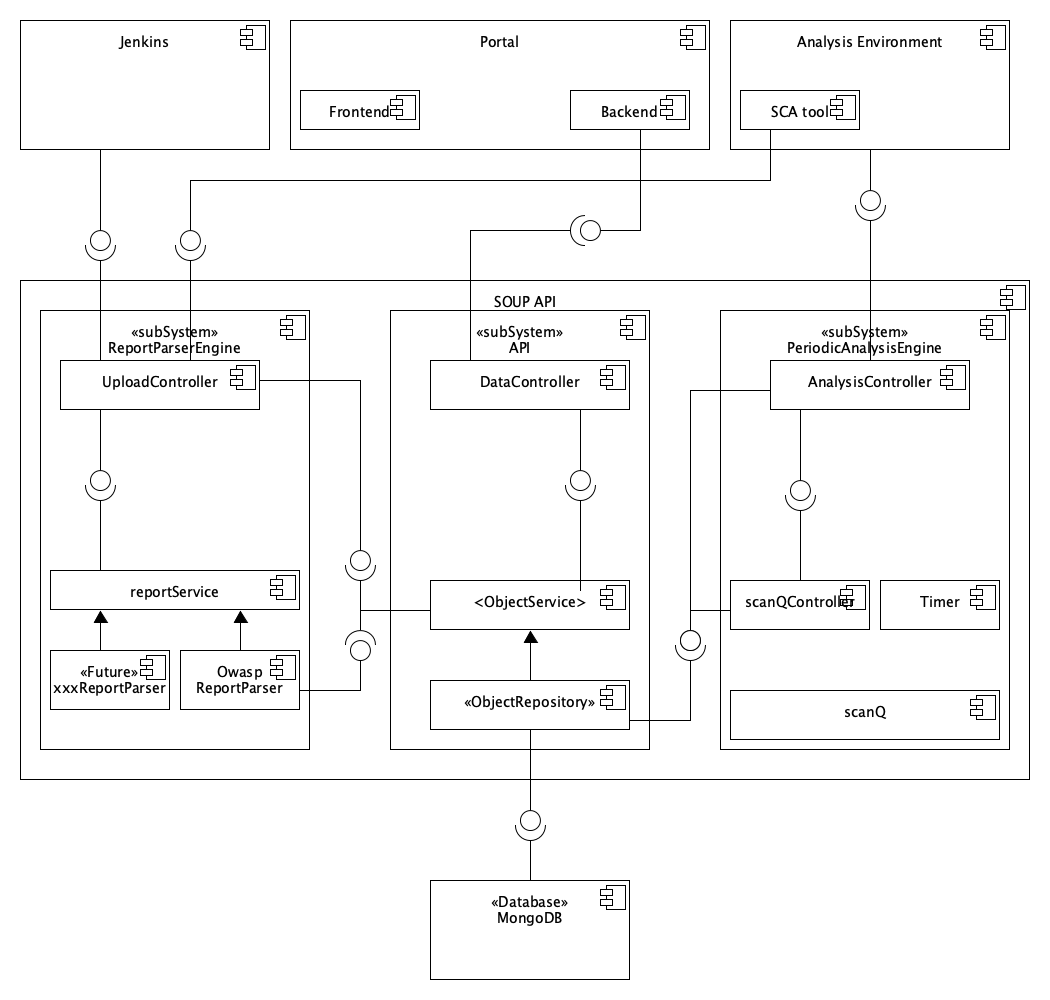
\includegraphics[width=10cm]{gfx/umlet/exports/ApplicationComponents}
    \caption{Componenten SOUP Analyse Systeem}
    \label{fig:SOUP-Components}
\end{figure}

% Afbeelding maken van alleen de SOUP API componenten
\section{SOUP API}\label{sec:soup-api} De SOUP API is het centrale deel van de applicatie.
Het is verantwoordelijk voor een aantal centrale zaken die nodig zijn voor het inzichtelijk maken van kwetsbaarheden binnen de projecten van Eaglescience.
De drie belangrijkste taken zijn de volgende:

Het \textbf{parsen} van binnen komende rapporten die door de SCA tooling is gemaakt. In het ontwerp is een parser opgenomen die een OWASP rapport omzet naar het interne datamodel. Echter is de opzet zo dat er in de toekomst meerdere tools kunnen worden gebruikt waar de SOUPAPI ook mee overweg moet kunnen.
Om met deze uitbreiding om te kunnen gaan is er een tussenlaag voorzien die het binnengekomen request bekijkt en er vervolgens de correcte parser bij zoekt. In het ontwerp is ook te zien dat er rapporten van twee verschillende processen komen. Als eerste jenkins Waarbij er naast het raport ook de dependencydeclaratiefiles worden meegestuurt welke worden gebruikt om een omgeving op te kunnen zetten voor de periodieke analyses. Het andere proces,  de periodeiek Analyses,  vertuurt alleen het rapport. De tussenlaag handeld ook dit verschil af door ervoor te zorgen dat de dependencyfiles worden verwerkt op het moment dat deze binnen komen.

De \textbf{PeriodicAnalysisEngine} is verantwoordelijk voor het uitvoeren van analyses op al bekende projecten op een ingestelde periode. Dit doet middels een scanQ waarin de modules staan die gescanned dienen te worden. Een controller is verantwoordelijk voor het aanbieden van de volgende analyseopdracht en de administratie binnen de ScanQ. De analysisController zorgt voor het daadwerkelijk uitvoeren van de analyse in een aparte docker omgeving.

De \textbf{API} is verantwoordelijk voor het dataverkeer met de portal, daarnaast bied het verschillende services aan die verantwoordelijk zijn mutaties in objcten die door de Repo wordt doorgevoerd naar de database.

\section{Jenkins}\label{sec:jenkins}
De bestaande jenkins omgeving is de primaire bron voor nieuwe informatie uit projecten. OP het moment dat er een deploy plaatsvind wordt er een analyse uitgevoerd welke samen met de dependency declaraties en metadata van het project worden verstuurt.

\section{Portal}\label{sec:portal} De portal is een inhouse applicatie welke gebruikt wordt voor administratieve zaken binnen het bedrijf. de wens is om hier functionaliteiten aan toe te voegen die bedrijfsbreed zijn en daarmee dus project oversteigend zijn. Voor deze applicatie dient er een module te worden toeegevoegd die fungeert als een interface waarin informatie over de bekende kwetsbaarheden te vinden is. maar ook instellingen kunnen worden

\section{Analysis Environment}\label{sec:analysis-environment}
Deze omgeving moet het mogelijk maken om vanuit de SOUP API een analyse uit te voeren op modulen. waarbij er een docker container wordt gestart een analyse uitgevoerd wordt en vervolgens de container wordt vernietigd. de voornaamste reden is dat er door de opzet van npm/node en sbt/scala veel combinatie kunnen ontstaan die ervoor kunnen zorgen dat er de versies die gebruikt worden veranderen. Om deze reden moet de analyse omgevingen een nagenoeg exacte kopie zijn van de omgeving op productie.


\section{Database}\label{sec:database} De gekozen database is nu MongoDB LATER MEER WELLICHT WORDT HET NOg MYSQL



\section{Dev-stack}\label{sec:dev-stack}

Om de applicatie te kunnen ontwikkelen is er voor de volgende dev-stack gekozen.

De SOUPAPI, backend van de server worden geschreven in Scala met het PlayFramework als webapplicatieFramework. De frontend van de portal wordt geschreven in Angular 13 omdat dit op dit moment ook wordt gebruikt voor de ontwikkeling van diezelfde portal en er is geen reden om dit te veranderen.
De keuze voor Scala met playframework en Angular lig voor de hand omdat dit al bekend is binnen de dev-stack van eaglescience.

De SOUP API zelf wordt in een docker container gedraaid.
